% Authors: Nelson Lago and Fernanda Magano
% This file is distributed under the MIT Licence

%%%%%%%%%%%%%%%%%%%%%%%%%%%%%%%%%%%%%%%%%%%%%%%%%%%%%%%%%%%%%%%%%%%%%%%%%%%%%%%%
%%%%%%%%%%%%%%%%%%%%%%%%%%%%%%%%% PREÂMBULO %%%%%%%%%%%%%%%%%%%%%%%%%%%%%%%%%%%%
%%%%%%%%%%%%%%%%%%%%%%%%%%%%%%%%%%%%%%%%%%%%%%%%%%%%%%%%%%%%%%%%%%%%%%%%%%%%%%%%

% aspectratio default é 4:3;
% as mais úteis são 169 (16:9), 1610 (16:10) e 149 (14:9)
% A língua padrão é a última citada
\documentclass[xcolor={usenames,svgnames,dvipsnames},brazil,english,12pt,aspectratio=149]{beamer}

% Funções auxiliares essenciais
\usepackage{etoolbox}
\usepackage{xstring}
\usepackage{xparse}
\usepackage{diagbox}
\usepackage{pifont}

% Vários pacotes e opções de configuração genéricos
\input{extras/basics}
% A fonte precisa ser definida depois que o tema metropolis foi carregado
%\input{extras/fonts}
\input{extras/floats}
% index não é necessário, mas deixamos aqui para usar os mesmos
% passos de compilação que a tese
\input{extras/index}
\input{extras/hyperlinks}
\input{extras/source-code}
\input{extras/utils}

% Diretório onde estão as figuras; com isso, não é preciso colocar o caminho
% completo em \includegraphics (e nem a extensão).
\graphicspath{{figuras/}}

% Comandos rápidos para mudar de língua:
% \en -> muda para o inglês
% \br -> muda para o português
% \texten{blah} -> o texto "blah" é em inglês
% \textbr{blah} -> o texto "blah" é em português
\babeltags{br = brazil, en = english}


%%%%%%%%%%%%%%%%%%%%%%%%%%%% APARÊNCIA DO BEAMER %%%%%%%%%%%%%%%%%%%%%%%%%%%%%%%

\usepackage{appendixnumberbeamer}

% Tema metropolis com algumas modificações
\dowithsubdir{extras/}{\usetheme{imeusp}}

% O padrão usa um tom de vermelho escuro como cor principal; a opção
% "greeny" troca essa cor por um tom de verde; a opção "sandy" usa o
% mesmo tom de verde mas modifica a cor padrão dos blocos para um
% tom amarelado.
\dowithsubdir{extras/}{\usecolortheme[greeny]{imeusp}}
% Desabilita a cor de rodapé
\setbeamercolor{footline}{fg=,bg=}

%%%%%%%%%%%%%%%%%%%%%%%%%% COMANDOS PARA O USUÁRIO %%%%%%%%%%%%%%%%%%%%%%%%%%%%%

\newcommand\col{\column{.5\textwidth}}

% A cada nova seção, recapitula o sumário
% Para desabilitar, é só comentar este trecho
\AtBeginSection[]{
  \begin{frame}<beamer>{Overview}
    \intermezzo
  \end{frame}
}

% Blocos de cor personalizada
\newenvironment{coloredblock}[2]%
{
    \setbeamercolor{block title}{fg=white,bg=#1!80!white}
    \setbeamercolor{block body}{fg=darkgray,bg=#1!20!white}
    \setbeamercolor{local structure}{fg=darkgray,bg=#1!20!white}
    \begin{block}{#2}
}{
    \end{block}
}

%%%%%%%%%%%%%%%%%%%%%%%%%%%%%%%%% METADADOS %%%%%%%%%%%%%%%%%%%%%%%%%%%%%%%%%%%%

% Referências
\usepackage[style=bwl-FU]{biblatex}
\addbibresource{bibliografia.bib}
% Acrescenta à lista de referências sem precisar incluir uma referência
% de fato no texto
\nocite{bronevetsky02,schmidt03:MSc, FSF:GNU-GPL, CORBA:spec, MenaChalco08}
% Acrescenta tudo do arquivo .bib
%\nocite{*}
\title[The shortened title]{Uma Visão Sobre a Próxima Geração de Abstrações de Processos em Sistemas Operacionais}
%\subtitle{The (optional) subtitle}

\author[Rodrigo Siqueira Jordão]{Rodrigo Siqueira Jordão}

\institute[USP]{\textbf{Orientador: Fabio Kon} \\ Instituto de Matemática e Estatística \\ IME USP}
%\institute[USP]{\textbf{Orientador:} \\ Computer Science Department \\ IME USP}

%\date{Month and day, year}

% Coloca a imagem no fundo da página de título
%\bgimage{\includegraphics[width=\paperwidth]{fundo_predios_e_grafo}}

% Logotipos no rodapé da página de título
\logos{
  \hfil\hfil\includegraphics[width=.1\textwidth]{usp-logo}\hfil%
  \raisebox{-.0103\paperheight}{\includegraphics[height=.0932\paperheight]{interscity-logo-branco}}\hfil%
%  \raisebox{-.00517\paperheight}{\includegraphics[height=.057\paperheight]{cnpq-logo}}\hfil%
  \raisebox{-.033\paperheight}{\includegraphics[width=.07\textwidth,trim=0 230 0 0,clip]{ime-logo}}\hfil\hfil
}

%\logos{
%  \hfil\hfil\includegraphics[width=.1\textwidth]{usp-logo}\hfil%
%  \raisebox{-.0103\paperheight}{\includegraphics[height=.0932\paperheight]{interscity-logo}}\hfil%
%  \raisebox{-.00517\paperheight}{\includegraphics[height=.057\paperheight]{cnpq-logo}}\hfil%
%  \raisebox{-.0342\paperheight}{\includegraphics[height=.1035\paperheight]{capes-logo}}\hfil%
%  \includegraphics[height=.044\paperheight]{fapesp-logo}\hfil\hfil
%}

% Usado para criar o qrcode com o endereço da apresentação
\presentationurl{https://siqueira.tech}

% Inclui o qrcode no sumário da apresentação
\includeqrcodeintoc

% O slide de sumário pode ser dividido em colunas; o parâmetro
% determina após qual o número da seção fazer a quebra de coluna
% (use zero para uma coluna ou simplesmente omita este comando).
\toccolumns{4}


%%%%%%%%%%%%%%%%%%%%%%%%%%%%%%%%%%%%%%%%%%%%%%%%%%%%%%%%%%%%%%%%%%%%%%%%%%%%%%%%
%%%%%%%%%%%%%%%%%%%%%%%%%%%% INÍCIO DA APRESENTAÇÃO %%%%%%%%%%%%%%%%%%%%%%%%%%%%
%%%%%%%%%%%%%%%%%%%%%%%%%%%%%%%%%%%%%%%%%%%%%%%%%%%%%%%%%%%%%%%%%%%%%%%%%%%%%%%%

\begin{document}

% É complicado colocar uma imagem de fundo, os logos das agências e
% o conteúdo "normal" do slide de título sem que as coisas fiquem
% bagunçadas, então definimos um comando para gerar o slide de título
\customtitlepage

% Slide com o qrcode
\showqrcode

% TODO: Sendo bem realista com o seu estilo de apresentação: vc quer manter esse slide? -> Resposta direta: NÃO!
%\begin{frame}{Sumário}
%  \overview
%\end{frame}
%
%\section{Introdução}
%\section{Fundamentação Teórica}
%\section{Validação de Novas Abstrações de Processos}
%\section{Estudo de Caso}
%\section{Análise Sobre Abstrações de Processos}
%\section{Conclusão}

%------------------------------------------------------------------------------
% FUNDAMENTAÇÃO TEÓRICA
%------------------------------------------------------------------------------
\begin{frame}[plain]
  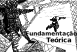
\includegraphics[width=\textwidth]{presentation_sec_one}
\end{frame}

% SUBSEÇÃO
\begin{frame}{Uma Breve Jornada Sobre os Processos}
	\begin{figure}[!h]
		\centering
		\includegraphics[width=.4\textwidth]{memory_segment} 
		\caption{Segmento de memória\label{fig:memory_segment}}
	\end{figure}
\end{frame}

\begin{frame}{Uma Breve Jornada Sobre os Processos}
	\begin{figure}[!h]
		\centering
		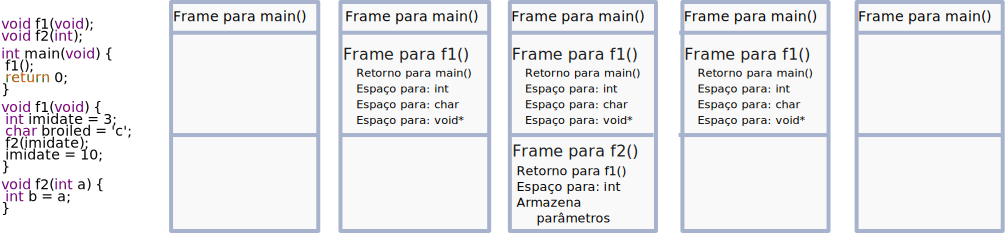
\includegraphics[width=\textwidth]{stack_frame}
		\caption{Alocação e desalocação de Stack frames considerando o padrão CDECL\label{fig:stack_frames}}
		%\caption{Alocação e desalocação de Stack frames considerando o padrão CDECL~\citep{patterson}\label{fig:stack_frames}}
	\end{figure}
\end{frame}

\begin{frame}{Uma Breve Jornada Sobre os Processos}
	\begin{figure}[!h]
		\centering
		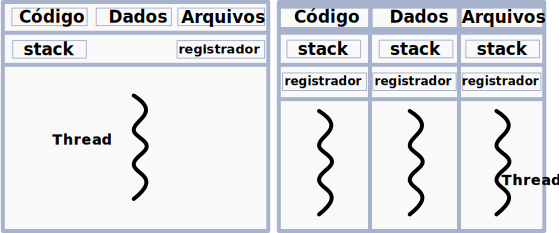
\includegraphics[width=.7\textwidth]{process_and_threads}
		\caption{Única thread e multi-thread. Note o isolamento da pilha e dos registrador (PC)\label{fig:single_thread_multi_thread}}
		%\caption{Única thread e multi-thread. Note o isolamento da pilha e dos registrador (PC)~\citep{silberschatz}\label{fig:single_thread_multi_thread}}
	\end{figure}
\end{frame}

\begin{frame}{Uma Breve Jornada Sobre os Processos}
	\begin{figure}[!h]
		\centering
		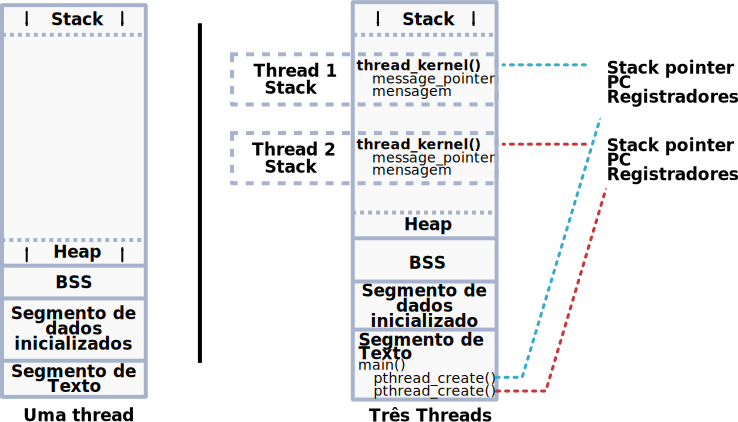
\includegraphics[width=.80\textwidth]{theads_and_stack} 
		\caption[Um processo com uma thread e um processo com três threads]{Um processo com uma thread (esquerda) e um processo com três threads (direita)\label{fig:stack_threads}}
	\end{figure}
\end{frame}

% SUBSEÇÃO
\begin{frame}{Gerenciamento da Memória Relacionada aos Processos}
	\begin{figure}[!h]
		\centering
		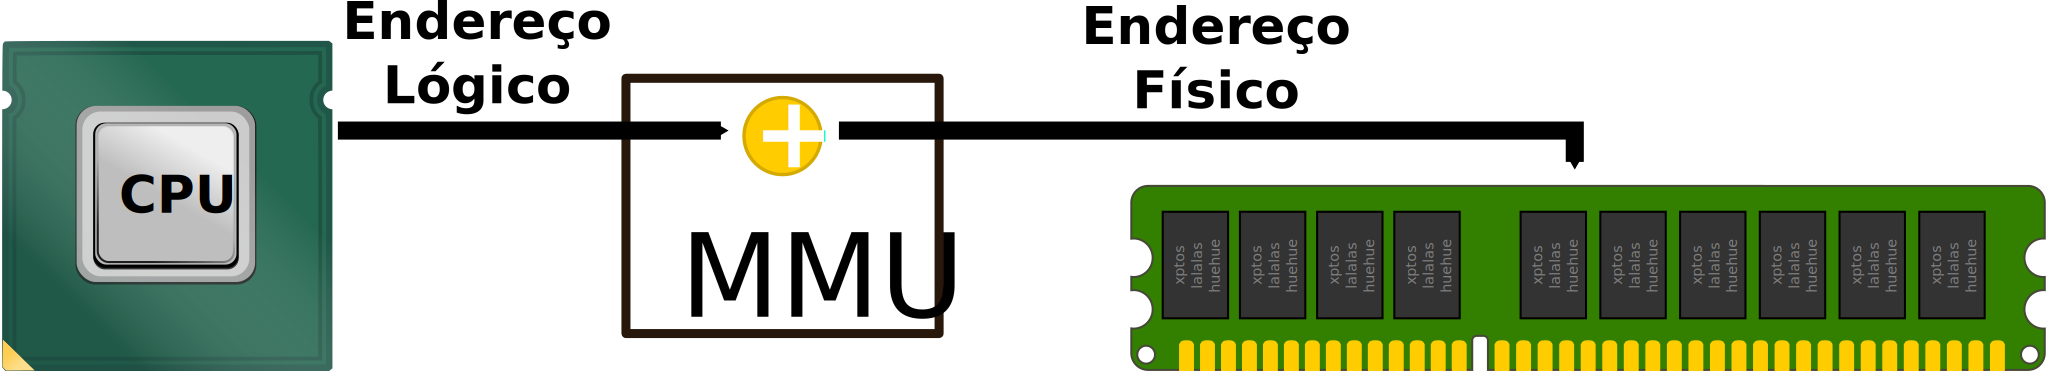
\includegraphics[width=\textwidth]{mmu} 
		\caption{Do endereço lógico ao físico com o auxílio da MMU}
		\label{fig:mmu}
	\end{figure}
\end{frame}

\begin{frame}{Gerenciamento da Memória Relacionada aos Processos}
	\begin{figure}[!h]
		\centering
		\includegraphics[width=.5\textwidth]{virtual_vs_fisico} 
		\caption{Espaço de endereçamento virtual vs. físico}
		\label{fig:vas_pas}
	\end{figure}
\end{frame}

\begin{frame}{O Modelo de Paginação}
	\begin{figure}[!h]
		\centering
		\includegraphics[width=0.8\textwidth]{paginacao} 
		\caption{Os elementos básicos presentes no modelo de paginação. Note que a busca na TLB e na tabela de página ocorre em paralelo}
		\label{fig:paginacao}
	\end{figure}
\end{frame}

\begin{frame}{O Modelo de Paginação}
	\begin{figure}[!h]
		\centering
		\includegraphics[width=\textwidth]{pte}
		\caption{entrada da tabela de páginas}
		\label{fig:pte}
	\end{figure}
\end{frame}

\begin{frame}{O Modelo de Paginação}
	\begin{figure}[!h]
		\centering
		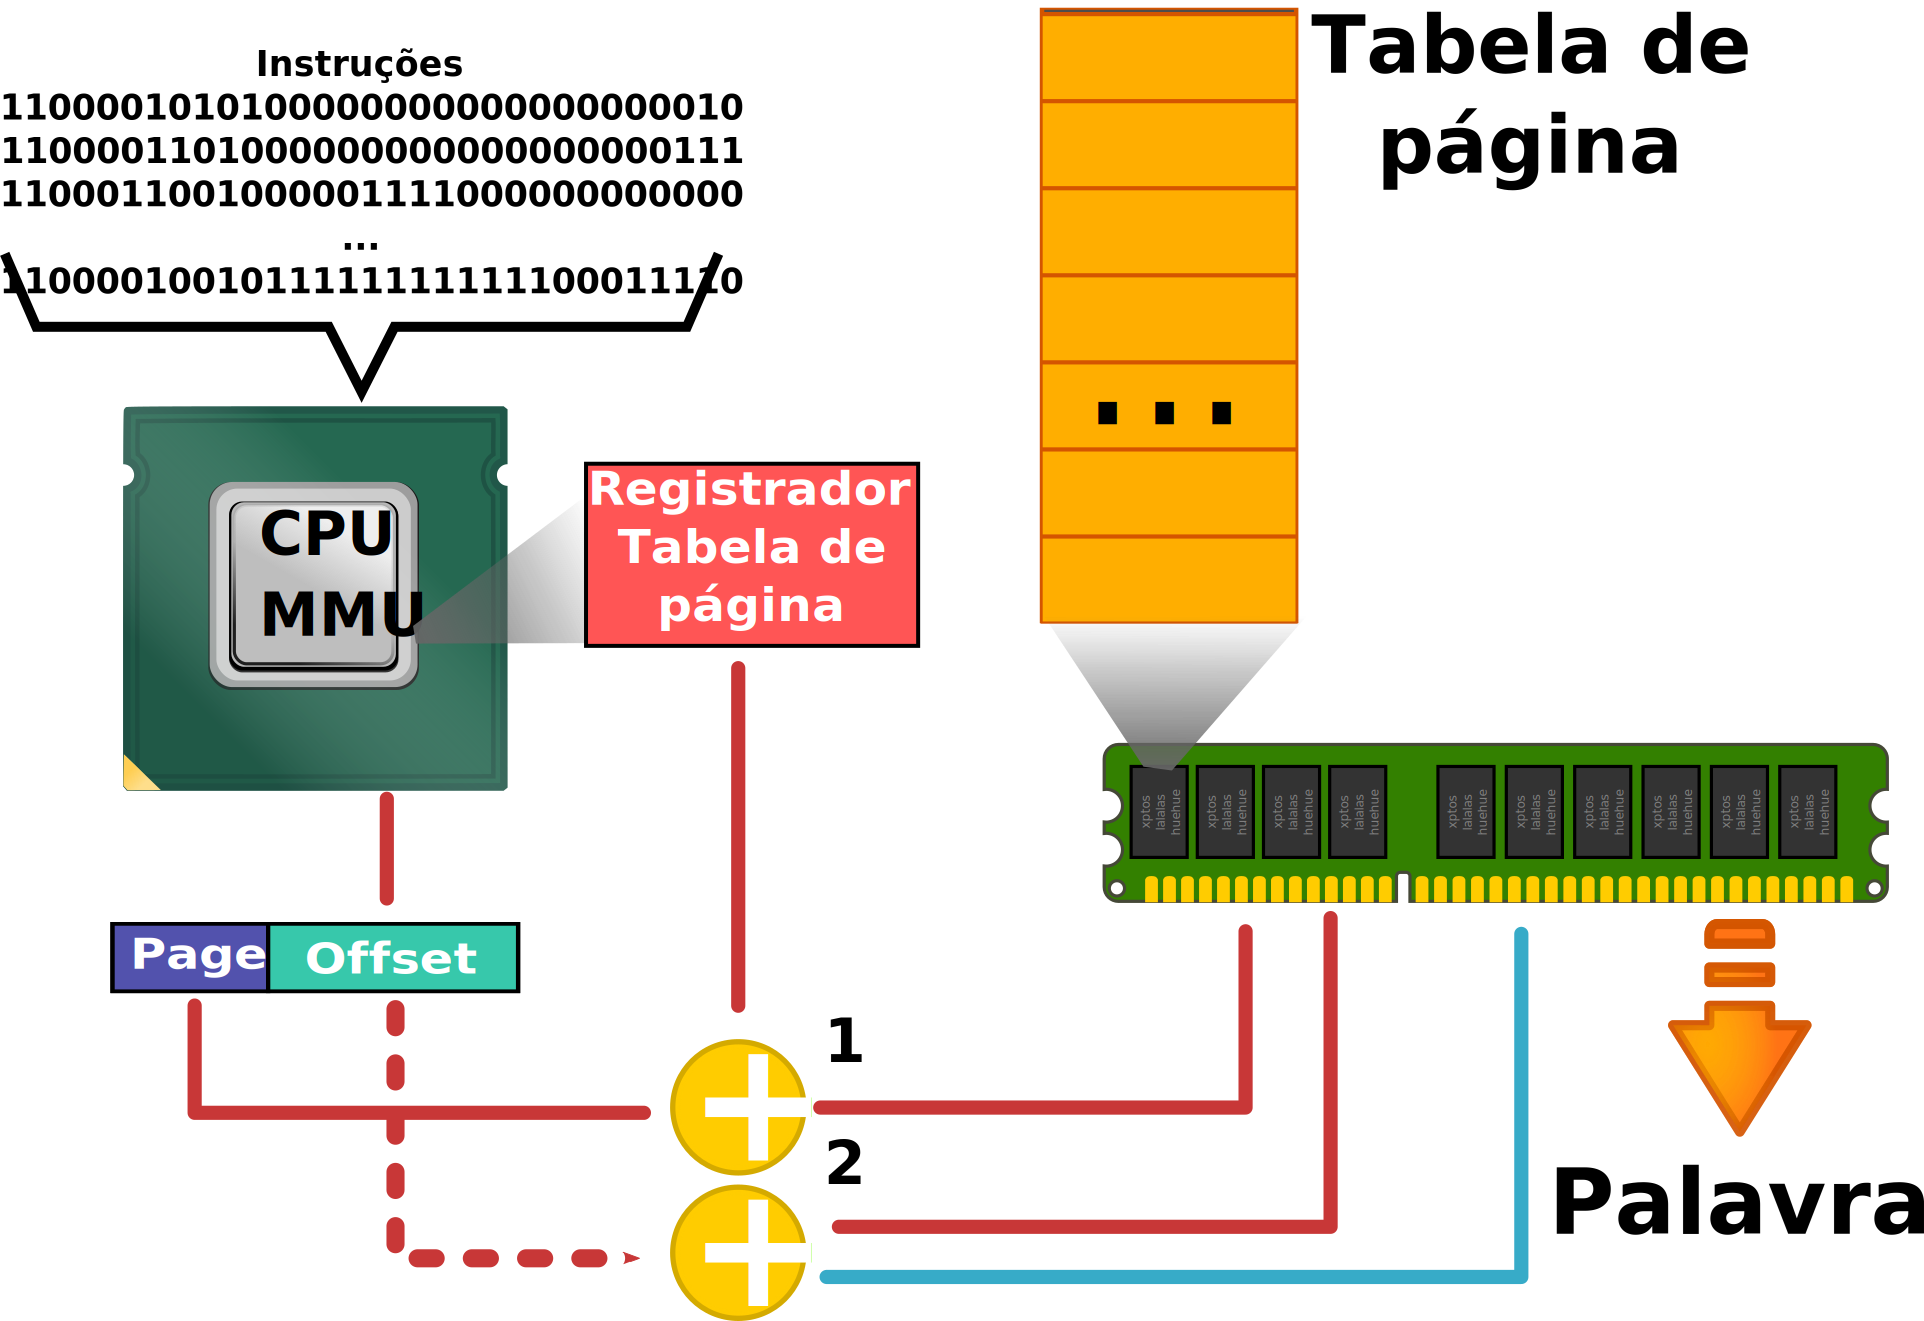
\includegraphics[width=0.8\textwidth]{paginacao_passos} 
		\caption{Passos do acesso a memória usando o modelo de paginação. A figura ilustra o caso simples na qual pelo menos dois acessos a memória são necessários}
		\label{fig:passos_paginacao}
	\end{figure}
\end{frame}

\begin{frame}{O Modelo de Paginação}
	\begin{figure}[!h]
		\centering
		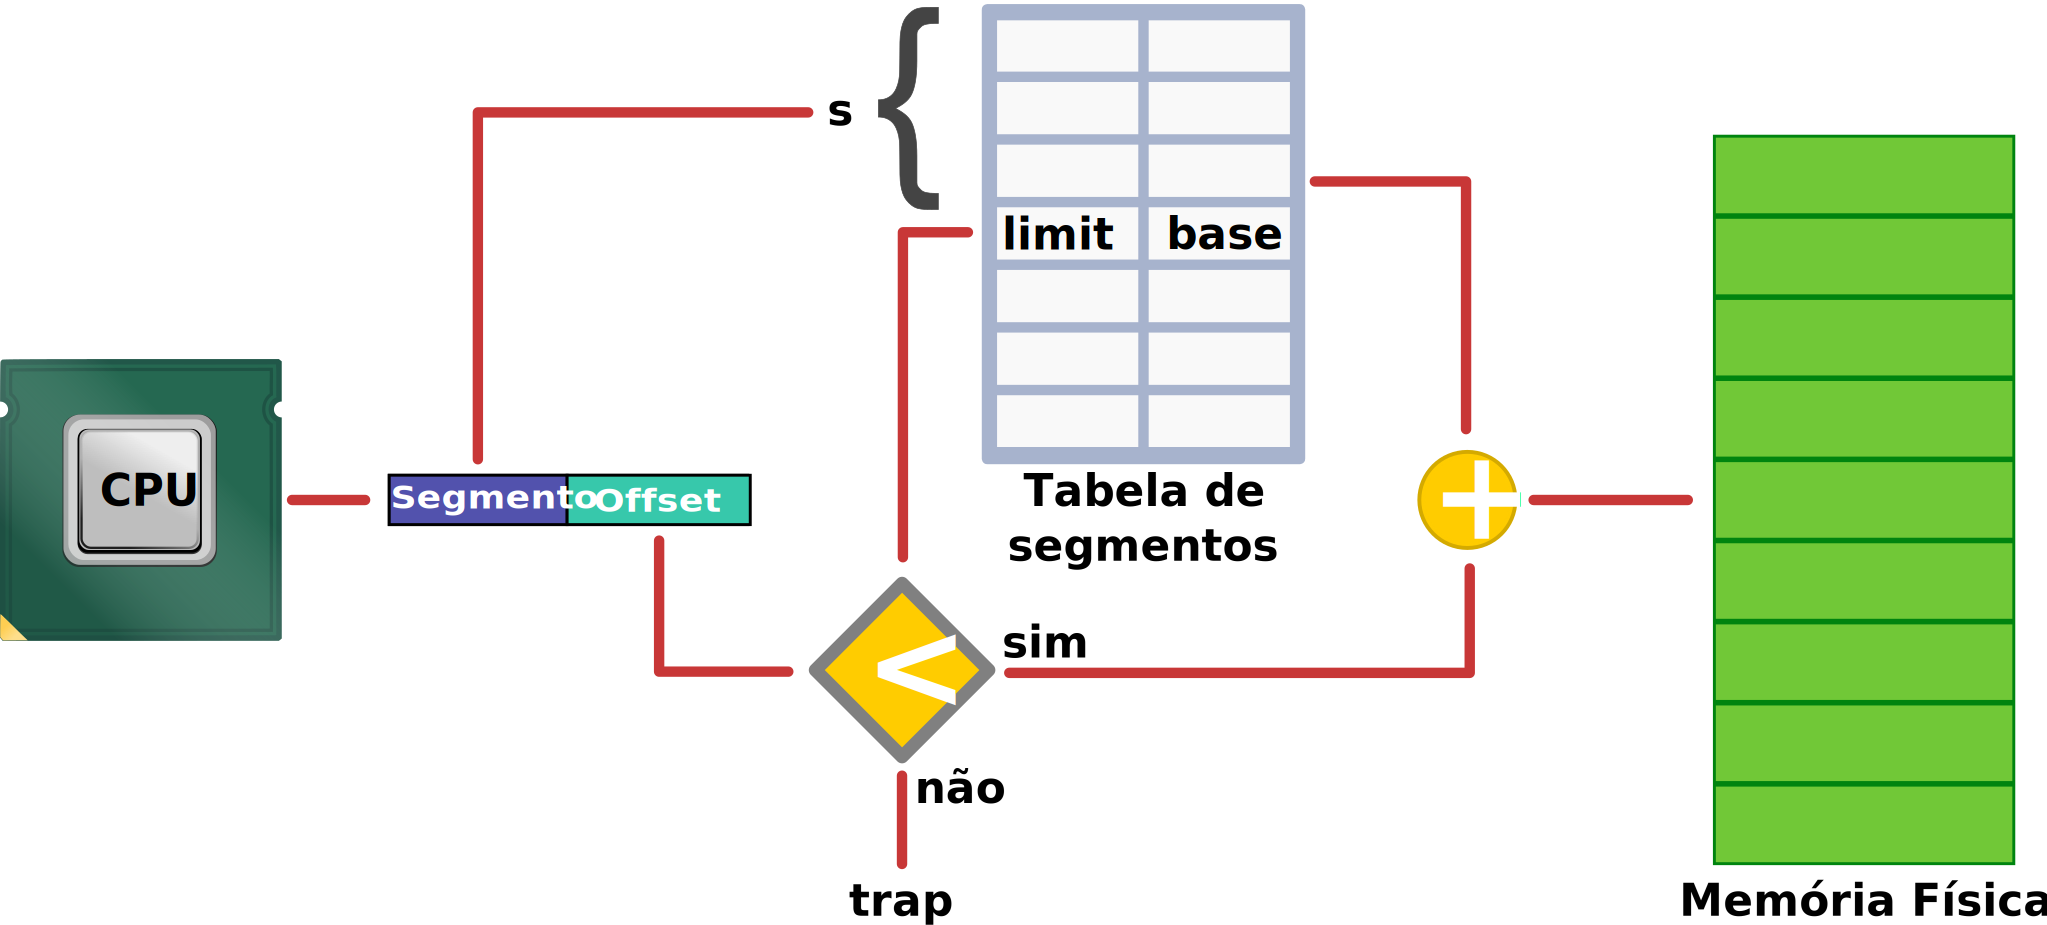
\includegraphics[width=.80\textwidth]{segmentacao} 
		\caption{Comportamento do modelo de segmentação. Note que a tabela de segmento é acessada para obter o valor base e esse é sempre verificado para evitar acessos indevidos a outras regiões da memória}
		\label{fig:segmentacao} 
	\end{figure}
\end{frame}

\begin{frame}{Proteção da memória}
	\begin{figure}[!h]
		\centering
		
\includegraphics[width=.80\textwidth]{pte_domain} 
		\caption{Ilustração de uma entrada da tabela de páginas utilizando novos bits}
		\label{fig:ptedominio} 
	\end{figure}
\end{frame}

\begin{frame}{Exemplo Prático Usando o GNU/Linux}
	\begin{figure}[!h]
		\centering
		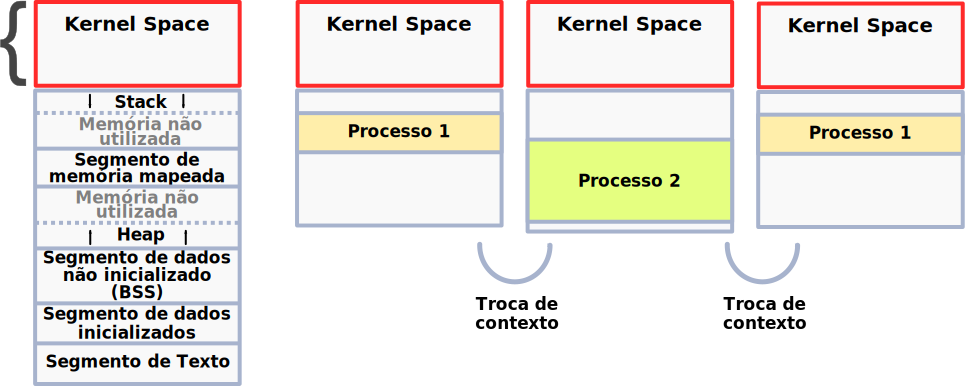
\includegraphics[width=\textwidth]{segmento_troca_contexto}
		\caption{VAS durante a troca de contexto}
		%\caption{VAS durante a troca de contexto~\citep{kernel_manage_mem}}
		\label{fig:vas_contexto}
	\end{figure}
\end{frame}

\begin{frame}{Exemplo Prático Usando o GNU/Linux}
	\begin{figure}[!h]
		\centering
		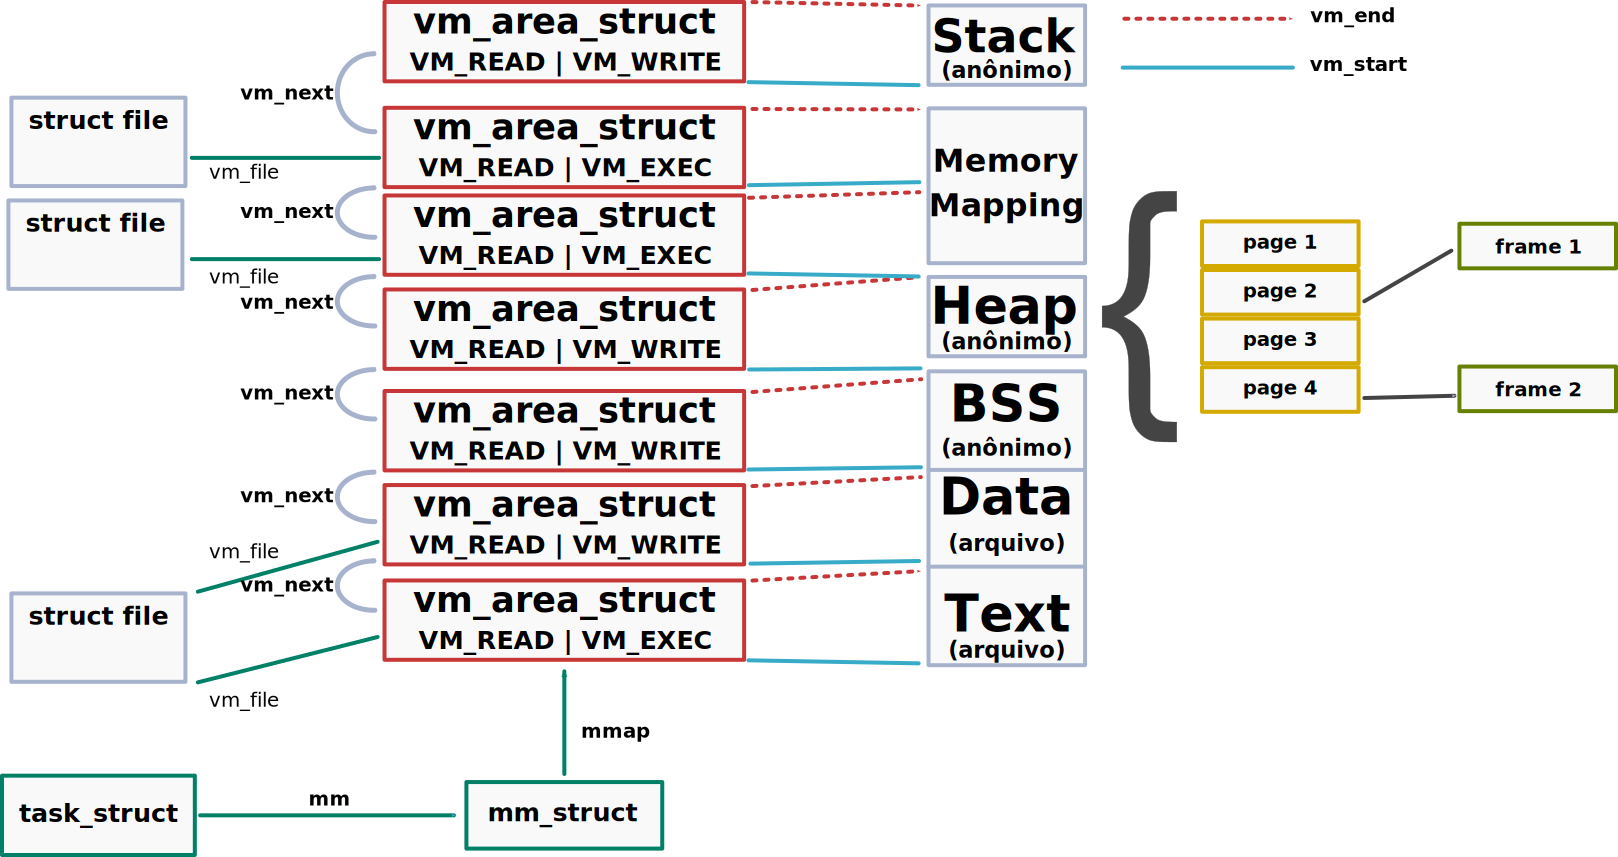
\includegraphics[width=.9\textwidth]{kernel_manages_memory}
		\caption{Visão interna do gerenciamento da memória}
		\label{fig:kernel_manages_memory}
	\end{figure}
\end{frame}

\begin{frame}{Exemplo Prático Usando o GNU/Linux}
	\begin{figure}[!h]
		\centering
		\includegraphics[width=\textwidth]{malloc}
		\caption{Passos envolvidos na alocação de memória com \texttt{malloc()}}
    % \caption[Passos envolvidos na alocação de memória com \texttt{malloc()}]{Passos envolvidos na alocação de memória com \texttt{malloc()} (imagem baseada em \cite{anatomy_program_mem})}
		\label{fig:malloc_linux}
	\end{figure}
\end{frame}

\begin{frame}{Chamadas de Sistema}
	\begin{figure}[!h]
		\centering
		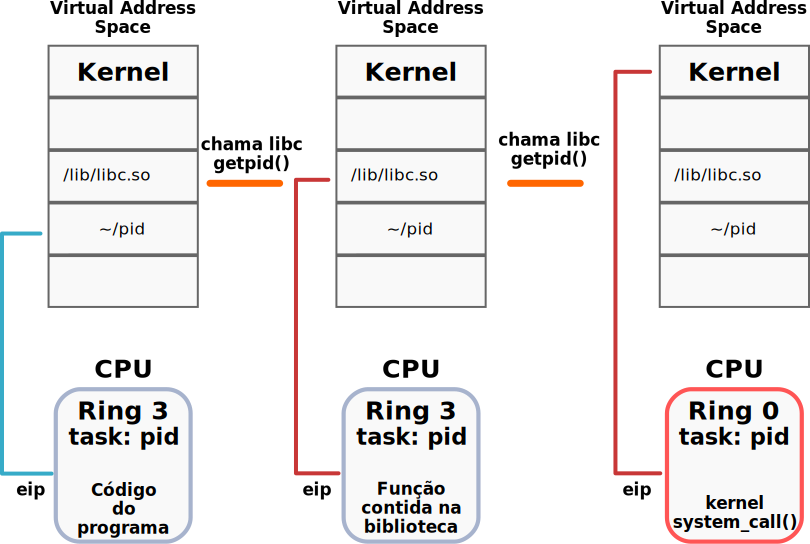
\includegraphics[width=0.5\textwidth]{userspace_to_kernel} 
		\caption{Execução do user space até o kernel space}
		\label{fig:userspace_kernelspace}
	\end{figure}
\end{frame}

\begin{frame}{Troca de Contexto}
\end{frame}

\begin{frame}{Descritores de Arquivo}
	\begin{figure}[!h]
		\centering
		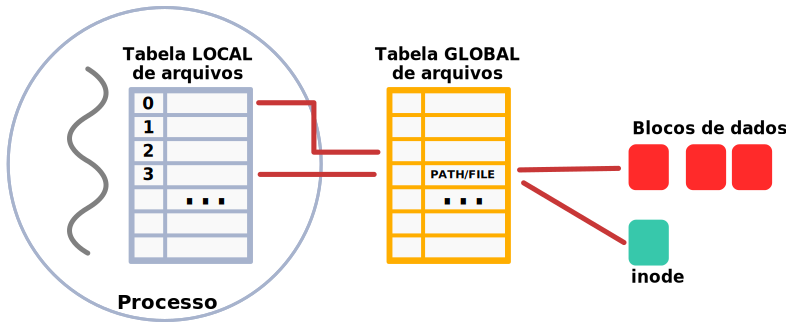
\includegraphics[width=.70\textwidth]{descritores} 
		\caption{Tabela local e global de arquivos}
		\label{fig:descritores} 
	\end{figure}
\end{frame}

\begin{frame}{Modelos de Programação}
\end{frame}

\begin{frame}{Aspectos de Implementação}
\end{frame}

\begin{frame}{Gerenciamento de Recursos}
\end{frame}

\begin{frame}{Outros Conceitos Indiretamente Relacionados a Abstração de Processos}
\end{frame}

\begin{frame}{Device Drivers}
\end{frame}

\begin{frame}{Virtualização}
	\begin{figure}[!h]
		\centering
		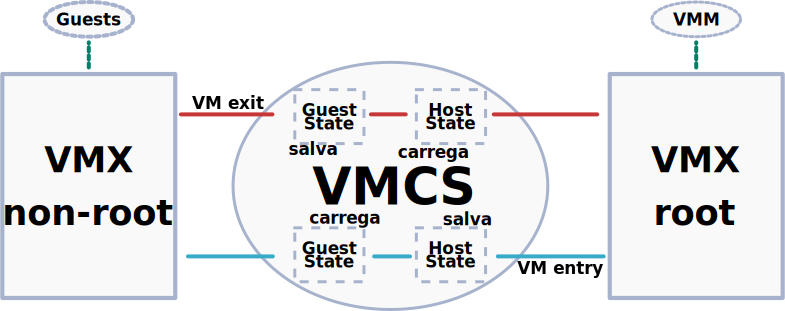
\includegraphics[width=0.7\textwidth]{vt-x_flow} 
		\caption{Fluxo do comportamento da tecnologia VT-x}
		\label{fig:vt-x_flow}
	\end{figure}
\end{frame}

\begin{frame}{A Tecnologia VT-x}
\end{frame}

%------------------------------------------------------------------------------
% Trabalhos Analisados
%------------------------------------------------------------------------------
% TODO: Slide de transição
\begin{frame}{Dune}
	\begin{figure}[!h]
		\centering
		\includegraphics[width=0.4\textwidth]{dune_architecture} 
		\caption[Arquitetura do Dune]{Arquitetura do Dune}
		%\caption[Arquitetura do Dune]{Arquitetura do Dune~\citep{belay}}
		\label{fig:dune_architecture}
	\end{figure}
\end{frame}

\begin{frame}{Shreds}
	\begin{figure}[!h]
		\centering
		\includegraphics[width=0.6\textwidth]{shreds} 
		\caption{Funcionamento geral do shreds}
		\label{fig:shreds}
	\end{figure}
\end{frame}

\begin{frame}{Wedge}
\end{frame}

\begin{frame}{Resource Container}
	\begin{figure}[!h]
		\centering
		\includegraphics[width=\textwidth]{resource_constainer_scenarios} 
		\caption{Cenários das aplicações}
		\label{fig:resource_constainer_scenarios}
	\end{figure}
\end{frame}

\begin{frame}{Nooks}
	\begin{figure}[!h]
		\centering
		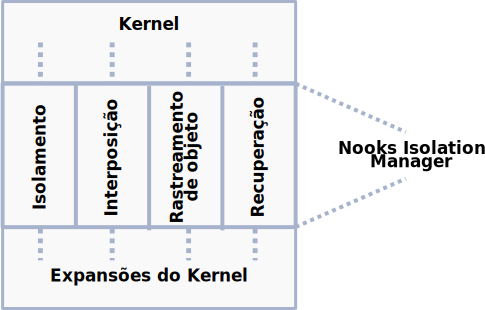
\includegraphics[width=0.8\textwidth]{nooks_nim}
		\caption[Visão geral da arquitetura do Nooks]{Visão geral da arquitetura do Nooks}
		%\caption[Visão geral da arquitetura do Nooks]{Visão geral da arquitetura do Nooks \citep{nooks}}
		\label{fig:nooks_nim}
	\end{figure}
\end{frame}

\begin{frame}{Nooks}
	\begin{figure}[!h]
		\centering
		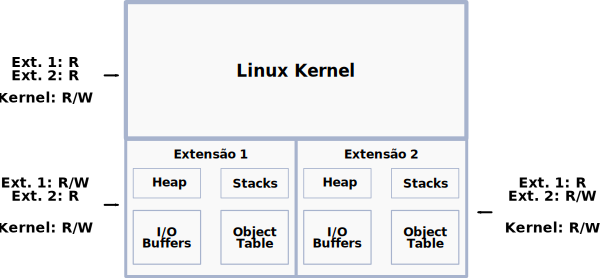
\includegraphics[width=0.8\textwidth]{nooks_mem}
		\caption[Acesso à memória do Nooks]{Acesso à memória do Nooks}
		%\caption[Acesso à memória do Nooks]{Acesso à memória do Nooks \citep{nooks}}
		\label{fig:nooks_mem}
	\end{figure}
\end{frame}

\begin{frame}{Mondrian Memory Protection e Mondrix}
	\begin{figure}[!h]
		\centering
		\includegraphics[width=0.7\textwidth]{mondrix_pd}
		\caption{Representação dos domínios de proteção do Mondrix}
		%\caption{Representação dos domínios de proteção do Mondrix (\cite{mondrix})}
		\label{fig:mondrixPD} 
	\end{figure}
\end{frame}

\begin{frame}{SpaceJMP}
	\begin{figure}[!h]
		\centering
		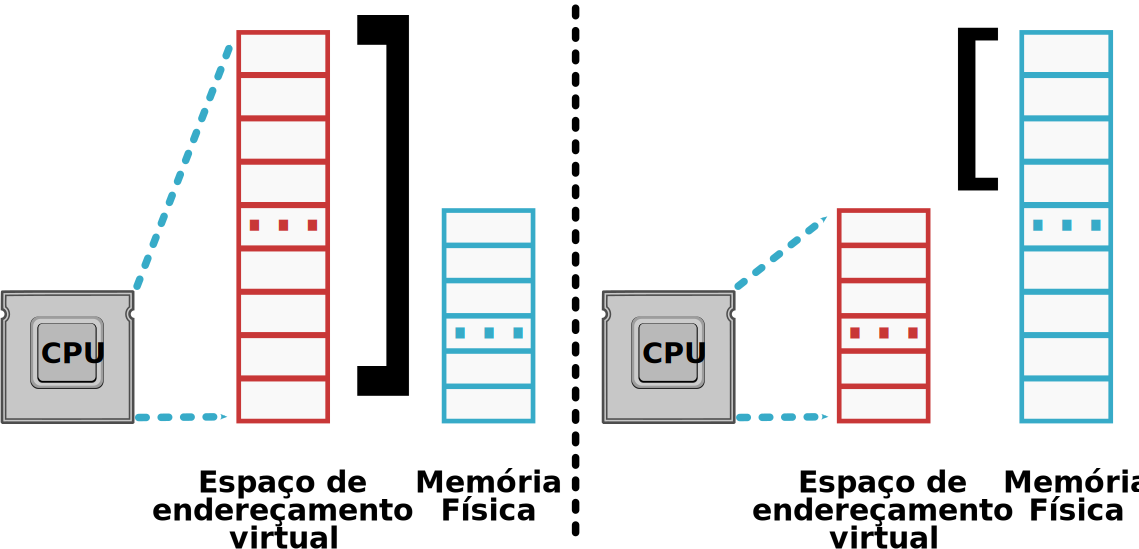
\includegraphics[width=.7\textwidth]{vas_vs_physical_address} 
		\caption{VAS e Memóra Física}
		\label{fig:vas_vs_physical} 
	\end{figure}
\end{frame}

\begin{frame}{SpaceJMP}
	\begin{figure}[!h]
		\centering
		\includegraphics[width=.7\textwidth]{solve_huge_address_memory}
		\caption{Resolvendo o problema de endereçar memórias físicas grandes}
		\label{fig:large_memory}
	\end{figure}
\end{frame}

\begin{frame}{SpaceJMP}
	\begin{figure}[!h]
		\centering
		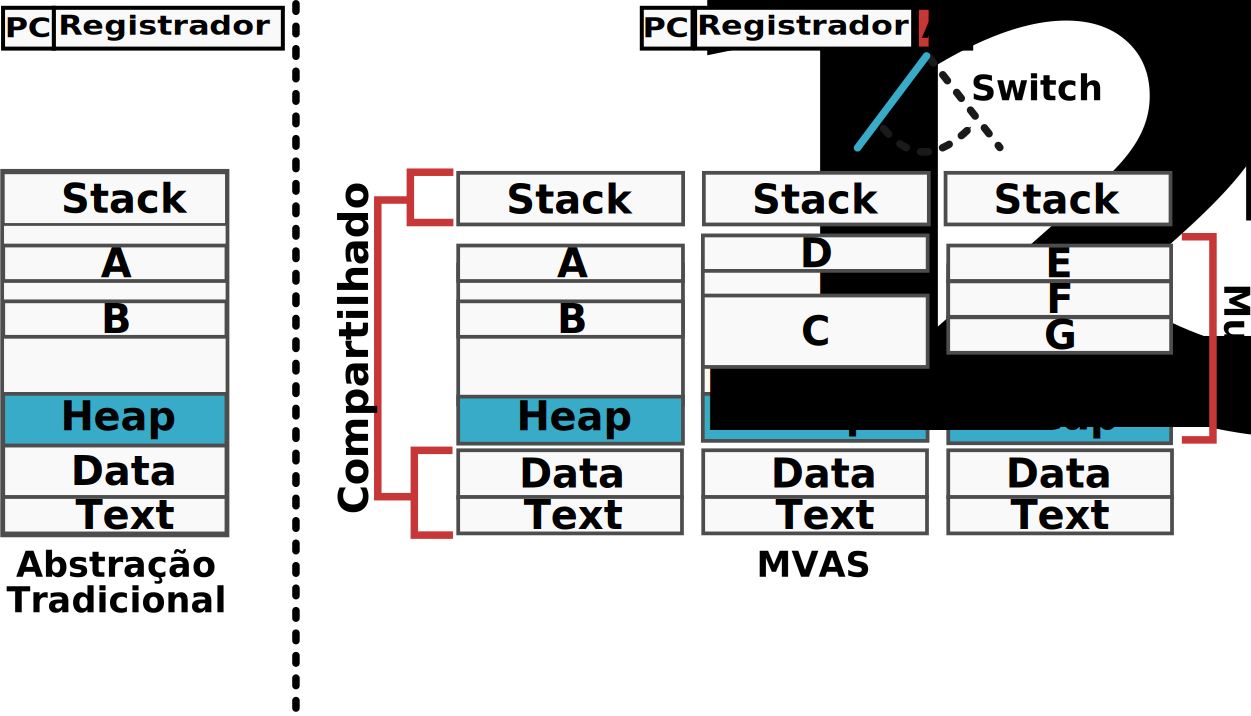
\includegraphics[width=.7\textwidth]{traditional_vs_mvas} 
		\caption{VAS e MVAS}
		%\caption{VAS e MVAS \citep{spacejmp}}
		\label{fig:traditional_vs_mvas} 
	\end{figure}
\end{frame}

\begin{frame}{SpaceJMP}
	\begin{figure}[!h]
		\centering
		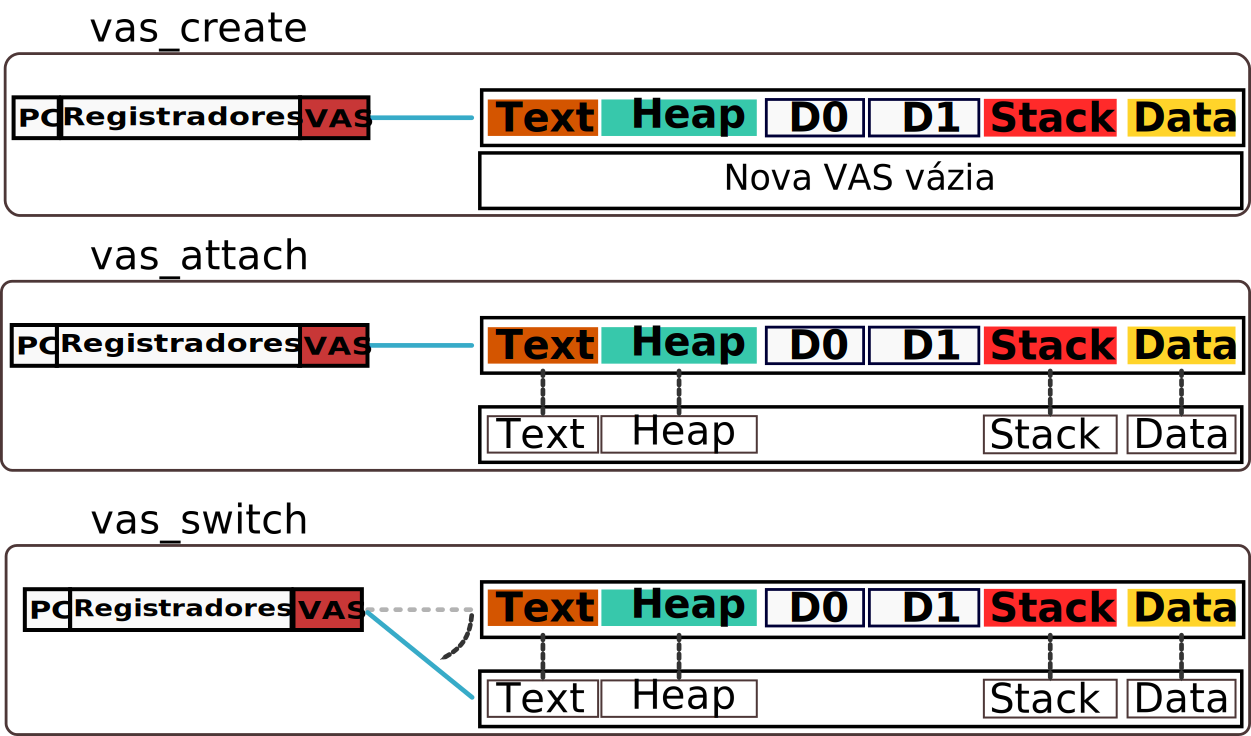
\includegraphics[width=.7\textwidth]{mvas_example} 
		\caption{System Call disponibilizada pelo SpaceJMP}
		%\caption{System Call disponibilizada pelo SpaceJMP \cite{ellarge}}
		\label{fig:mvas_example}
	\end{figure}
\end{frame}

\begin{frame}{Light-weight Contexts}
	\begin{figure}[!h]
		\centering
		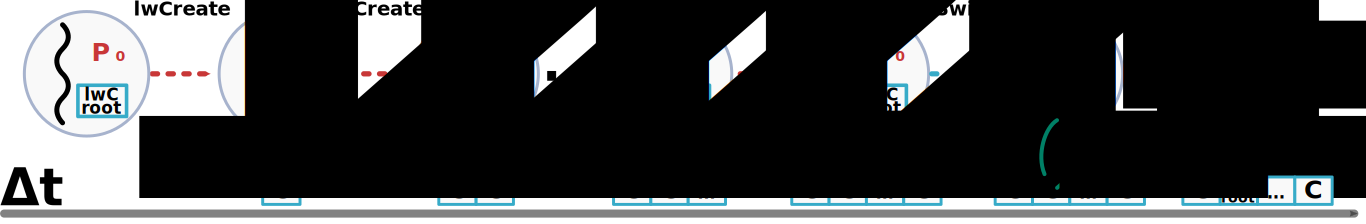
\includegraphics[width=\textwidth]{lwC} 
		\caption{Exemplo do comportamento do lwC}
		\label{fig:lwc} 
	\end{figure}
\end{frame}

\begin{frame}{Exokernel}
\end{frame}

%------------------------------------------------------------------------------
% Validação de Novas Abstrações de Processos
%------------------------------------------------------------------------------
\begin{frame}{Servidores Web}
	\begin{figure}[!h]
		\centering
		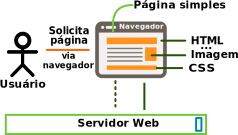
\includegraphics[width=.50\textwidth]{request_a_page}
		\caption{Do cliente para o servidor Web.}
		\label{fig:client_to_web_server}
	\end{figure}
\end{frame}

\begin{frame}{Servidores Web}
	\begin{figure}[!h]
		\centering
		
\includegraphics[width=0.8\textwidth]{keep_alive}
		\caption{Com keep alive}
		\label{fig:keep_alive}
	\end{figure}
\end{frame}

\begin{frame}{Servidores Web}
	\begin{figure}[!h]
		\centering
		
\includegraphics[width=0.8\textwidth]{no_keep_alive}
		\caption{Sem keep alive}
		\label{fig:no_keep_alive}
	\end{figure}
\end{frame}

\begin{frame}{Servidor Apache HTTPD}
	\begin{figure}[!h]
		\centering
		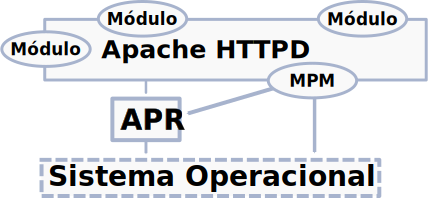
\includegraphics[width=.7\textwidth]{apache_arhitecture} 
		\caption{Arquitetura do servidor Apache HTTP}
		\label{fig:apache_architecture} 
	\end{figure}
\end{frame}

\begin{frame}{Servidor Apache HTTPD}
	\begin{figure}[!h]
		\centering
		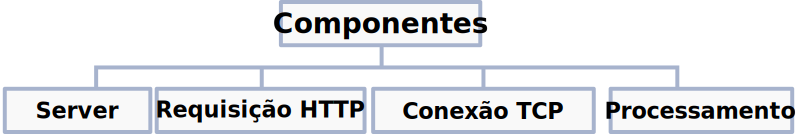
\includegraphics[width=.7\textwidth]{units} 
		\caption{Unidade do Servidor Apache HTTP}
		\label{fig:units} 
	\end{figure}
\end{frame}

\begin{frame}{Servidor Apache HTTPD}
	\begin{figure}[!h]
		\centering
		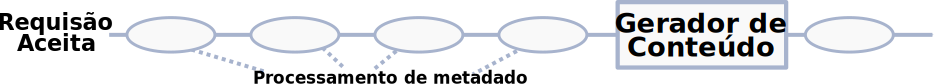
\includegraphics[width=.9\textwidth]{request_phases} 
		\caption{Gerador de Conteúdo}
		%\caption[Gerador de Conteúdo]{Gerador de Conteúdo \citep{apache_module_book}}
		\label{fig:content_generator} 
	\end{figure}
\end{frame}

\begin{frame}{Servidor Apache HTTPD}
	\begin{figure}[!h]
		\centering
		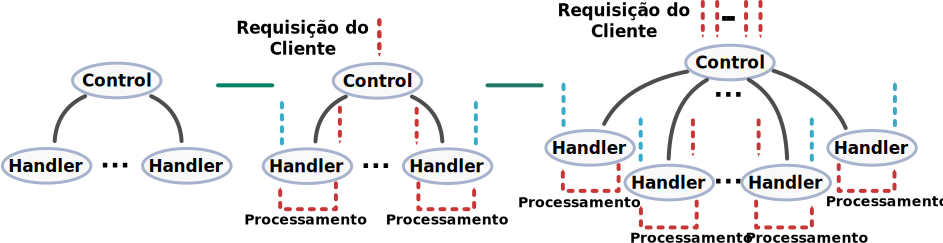
\includegraphics[width=\textwidth]{prefork} 
		\caption{Prefork}
		\label{fig:prefork} 
	\end{figure}
\end{frame}

\begin{frame}{Servidor Apache HTTPD}
	\begin{figure}[!h]
		\centering
		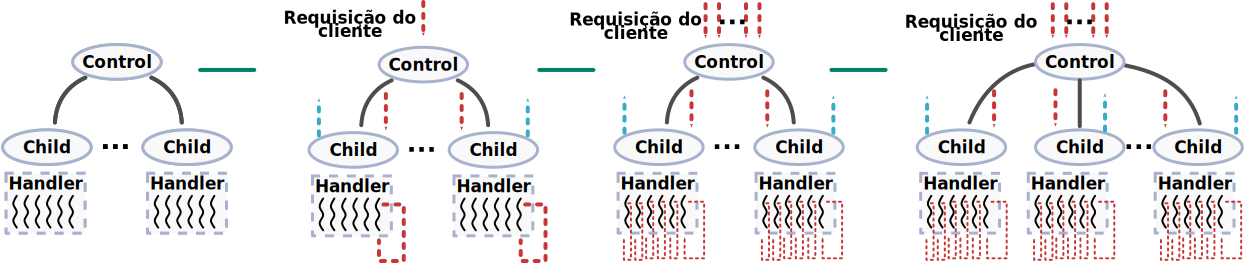
\includegraphics[width=\textwidth]{worker} 
		\caption{Worker}
		\label{fig:worker} 
	\end{figure}
\end{frame}

\begin{frame}{Servidor Apache HTTPD}
	\begin{figure}[!h]
		\centering
		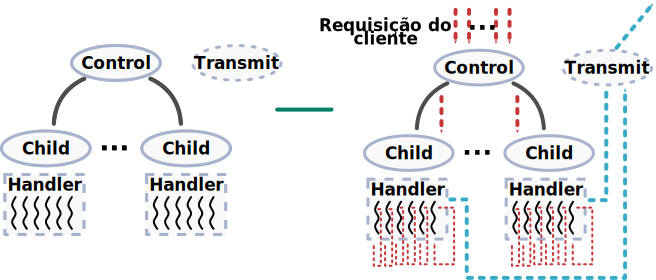
\includegraphics[width=.7\textwidth]{event} 
		\caption{Event}
		\label{fig:event} 
	\end{figure}
\end{frame}

\begin{frame}{Nginx}
	\begin{figure}[!h]
		\centering
		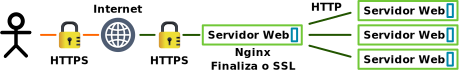
\includegraphics[width=\textwidth]{nginx_load_balancer_ex} 
		\caption{Nginx comportando-se como reverse-proxy}
		%\caption[Nginx comportando-se como reverse-proxy]{Nginx comportando-se como reverse-proxy \citep{soni}}
		\label{fig:nginx_basico} 
	\end{figure}
\end{frame}

\begin{frame}{Ferramentas de Comunicação Criptografada}
\end{frame}

\begin{frame}{OpenSSL}
	\begin{figure}[!h]
		\centering
		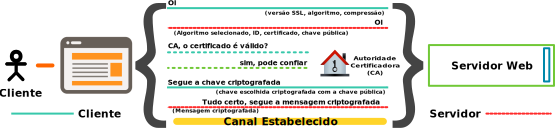
\includegraphics[width=\textwidth]{ssl_handshake}
		\caption{Do cliente para o servidor Web}
		\label{fig:openssl_handshake}
	\end{figure}
\end{frame}

\begin{frame}{OpenSSL}
	\begin{figure}[!h]
		\centering
		\includegraphics[width=\textwidth]{openssl_arch}
		\caption{Arquitetura do OpenSSL}
		\label{fig:openssl_arch}
	\end{figure}
\end{frame}

\begin{frame}{OpenSSH}
	\begin{figure}[!h]
		\centering
		\includegraphics[width=0.3\textwidth]{ssh_layers}
		\caption{Camadas SSH}
		%\caption[Camadas SSH]{Camadas SSH \citep{opensshhood}}
		\label{fig:openssh_layer}
	\end{figure}
\end{frame}

\begin{frame}{Outras Aplicações}
\end{frame}

\begin{frame}{Redis}
	\begin{figure}[!h]
		\centering
		\includegraphics[width=\textwidth]{redis_overview}
		\caption{Visão geral do funcionamento do Redis}
		\label{fig:redis}
	\end{figure}
\end{frame}

\begin{frame}{Garbage Collection (GC)}
	\begin{figure}[!h]
		\centering
		\includegraphics[width=\textwidth]{gc_algoritmo}
		\caption{Algoritmo de pintura da memória}
		%\caption[Algoritmo de pintura da memória]{Algoritmo de pintura da memória\citep{gc_basics}}
		\label{fig:gc_alg}
	\end{figure}
\end{frame}

\begin{frame}{Garbage Collection (GC)}
	\begin{figure}[!h]
		\centering
		\includegraphics[width=0.8\textwidth]{gc_memory}
		\caption{Visão da memória durante a aplicação do algoritmo de GC}
		%\caption[Visão da memória durante a aplicação do algoritmo de GC]{Visão da memória durante a aplicação do algoritmo de GC\citep{gc_basics}}
		\label{fig:gc_mem}
	\end{figure}
\end{frame}

\begin{frame}{Discussão Sobre as Aplicações}
	\begin{table}[]
\small
\centering
  \begin{tabular}{|@{}c@{}|@{}c@{}|@{}c@{}|@{}c@{}|@{}c@{}|@{}c@{}|@{}c@{}|}
  % TOPO DA TABELA
  % |M{2.5cm}|M{2.5cm}|M{2.5cm}|
  \hline
  \multicolumn{1}{|l|}{\diagbox[width=2.5cm, height=2cm]{App}{Alvo}} &
    % Troca de contexto
    \multicolumn{1}{@{}c@{}|}{\begin{tabular}[c]{@{}c@{}}Controle\\fino da\\Memória\end{tabular}} &
    % Persistência de processos
    \multicolumn{1}{@{}c@{}|}{\begin{tabular}[c]{@{}c@{}}Consumo\\ de CPU \end{tabular}} &
    % Controle fino de privilégios
    \multicolumn{1}{@{}c|}{\begin{tabular}[c]{@{}c@{}}Consumo \\de Memória \end{tabular}} &
    % Segurança
    \multicolumn{1}{@{}c|}{Segurança} &
    % Recuperação
    \multicolumn{1}{@{}c|}{Recuperação} &
    % Otimização
    \multicolumn{1}{@{}c|}{Otimização} \\ \hline \hline
  % Início da tabela
  Apache                                                                    & \ding{52}\ding{52}\ding{52} &                    & & & & \ding{52}\ding{52} \\ \hline
  Nginx                                                                   & \ding{52}\ding{52}          & \ding{52}\ding{52} & & & \ding{52}\ding{52} & \\ \hline
  OpenSSL                                                         &                             &                    & & \ding{52} & & \ding{52}\ding{52}\ding{52} \\ \hline
  OpenSSH                                                           & \ding{52}\ding{52}          &                    & \ding{52}\ding{52}\ding{52} & \ding{52}\ding{52} & & \\ \hline
  Redis                                                           &                             &                    & & \ding{52}\ding{52}\ding{52} & \ding{52}\ding{52}\ding{52} & \\ \hline
  GC                                                           &                             &                    & & \ding{52}\ding{52}\ding{52} & \ding{52}\ding{52}\ding{52} & \\ \hline
  \end{tabular}
\caption{Relação aplicações e alvos}
\label{tab:app_alvos}
\end{table}

\end{frame}

\begin{frame}{Microbenchmarks}
\end{frame}

\begin{frame}{Discussão}
	\begin{quote}
		\item \emph{QP3:.} ``Quais aplicações podem ser utilizadas para avaliar as novas abstrações adicionadas ao SO?''
		\item \emph{QP4:.} ``Qual conjunto de \emph{microbenchmarks} pode ser utilizado para auxiliar a entender os impactos de uma nova característica adicionada às abstrações de processos?''
	\end{quote}
\end{frame}

%------------------------------------------------------------------------------
% Estudo de caso
%------------------------------------------------------------------------------
\begin{frame}{Estudo de Caso}
\end{frame}

\begin{frame}{Metodologia}
	\begin{figure}[!h] \centering
		\includegraphics[width=.60\textwidth]{web_server_organization_strategy}
		\caption{Visão geral da organização de aplicações utilizando servidores Web}
	\label{fig:web_server} \end{figure}
\end{frame}

\begin{frame}{Metodologia}
	\begin{figure}[!h] \centering
		\includegraphics[width=.90\textwidth]{experiment_arhitecture}
		\caption{Arquitetura do experimento} \label{fig:experiment_architecture}
	\end{figure}
\end{frame}

\begin{frame}{Customizações no Servidor Apache e no GNU/Linux}
	\begin{table}
  \centering
  \begin{tabular}{|c|c|c|c|}
  \hline
    \textit{Parameter} & \textbf{Event} & \textbf{Worker} & \textbf{Prefork} \\
      \hline\hline
    \textbf{ServerLimit} & 6000 & 6000 & 5000\\
      \hline
    \textbf{StartServer} & 10 & 10 & 1000\\
      \hline
    \textbf{MinSpareThreads} & 512 & 512 & --\\
      \hline
    \textbf{MaxSpareThreads} & 1024 & 1024 & --\\
      \hline
    \textbf{ThreadLimit} & 64 & 64 & --\\
      \hline
    \textbf{ThreadPerChild} & 64 & 64 & --\\
      \hline
    \textbf{MaxRequestWorkers} & 5120 & 5120 & 5000\\
      \hline
    \textbf{MinSpareServers} & -- & -- & 500\\
      \hline
    \textbf{MaxSpareServers} & -- & -- & 1500\\
      \hline
  \end{tabular}

  \caption{Configuração adotada para o MPM}
  \label{tab:configuration}

\end{table}


\end{frame}

\begin{frame}{Customizações no Servidor Apache e no GNU/Linux}
	\begin{table}
  \centering
  \begin{tabular}{|c|c|} \hline
  \textit{parameter} & \textbf{value}\\
    \hline\hline
   Max queue events & 1048576\\
     \hline
   Max user instances & 1048576\\
    \hline
   Max user watches & 1048576\\
    \hline
   Max map count & 262144\\
    \hline
   TCP max syn backlog & 8096\\
    \hline TCP syncookies & 0\\
    \hline
  \end{tabular}

  \caption{Configurações feitas no Kernel}
  \label{tab:kernel_config}
\end{table}


\end{frame}

\begin{frame}{Cenário}
	\begin{table}[!h]
  \centering
  \begin{tabular}{|c|c|c|}
      \hline 
    & \textbf{Pequeno} & \textbf{Grande}\\
      \hline\hline
    Static & 70Kb & 120Kb\\
      \hline
    Dynamic & 80Kb & 120Kb \\
      \hline
  \end{tabular}

  \caption{Tamanho dos arquivos para serem transferidos}
  \label{tab:file_size}
\end{table}


\end{frame}

\begin{frame}{Cenário}
	\begin{table}[h!]
  \centering
  \begin{tabular}{|c|c|c|}
      \hline
    Casos & \textbf{Requisições} & \textbf{Concorrência}\\
      \hline\hline
    Arquivos estáticos & 60000 & 20000\\
      \hline
    Arquivos dinâmicos & 5000 & 600 \\
      \hline
  \end{tabular}
  \caption{Carga principal aplicada}
  \label{tab:loads}
\end{table}


\end{frame}

\begin{frame}{MVAS Dentro do GNU/Linux e Apache HTTP Server}
	\begin{figure}[!h]
		\centering
		\includegraphics[width=\textwidth]{mvas_httpd}
		\caption{HTTPD com MVAS}
		\label{fig:httpd_mvas}
	\end{figure}
\end{frame}

\begin{frame}{Resultados}
	\begin{table}[h!]
  \centering
  \begin{tabular}{|c|c|c|}
      \hline
    Nome & \textbf{Núcleo} & \textbf{Memória}\\
      \hline
    M1 & 2 & 13Gb \\
      \hline
    M2 & 2 & 4Gb \\
      \hline
   \end{tabular}

  \caption{Hardware}
  \label{tab:machines}
\end{table}


\end{frame}

\begin{frame}{Resultados}
	\begin{figure}[!h]
		\centering
		\includegraphics[width=.60\textwidth]{static_file}
		\caption{Arquivos estáticos: tempo gasto para servir o percentual de requisições}
		\label{fig:static_file}
	\end{figure}
\end{frame}

\begin{frame}{Resultados}
	\begin{figure}[!h]
		\centering
		\includegraphics[width=.70\textwidth]{static_file_memory_usage}
		\caption{Arquivos estáticos: O consumo de memória necessário para atender todas as requisições}
		\label{fig:static_file_memory}
	\end{figure}
\end{frame}

\begin{frame}{Resultados}
	\begin{figure}[!h]
		\centering
		\includegraphics[width=.60\textwidth]{dynamic_file_request_time}

		\caption{Arquivos Dinâmicos: Tempo gasto por percentual de requisições}
		\label{fig:dynamic_file}
	\end{figure}
\end{frame}

\begin{frame}{Resultados}
	\begin{figure}[!h]
		\centering
		\includegraphics[width=.60\textwidth]{dynamic_file_memory_usage}

		\caption{Arquivos Dinâmicos: Consumo de memória necessário para servir as requisições}
		\label{fig:dynamic_file_memory}
	\end{figure}
\end{frame}

\begin{frame}{Discussão Sobre os Experimentos}
\end{frame}

%------------------------------------------------------------------------------
% Análise Sobre Abstrações de Processos
%------------------------------------------------------------------------------
\begin{frame}{Análise Sobre Abstrações de Processos}
\end{frame}

\begin{frame}{Análise Sobre Abstrações de Processos}
	\begin{quote}
	 \item \textit{QP1:.} ``Quais são as características desejáveis para a próxima geração de abstrações de processos?''
	 \item \textit{QP2:.} ``Quais são os principais desafios em se implementar a próxima geração de abstrações de processos?''
	\end{quote}
\end{frame}

\begin{frame}{Potenciais e Dificuldades Para a Adoção de Novas Abstrações de Processos}
	\begin{table}[]
\small
\centering

\begin{tabular}{|@{}c@{}|@{}c@{}|@{}c@{}|@{}c@{}|@{}c@{}|@{}c@{}|@{}c|c@{}|@{}c@{}|}
% HEADERS
\hline
  \multirow{2}{*}{Trabalho}          &
  \multicolumn{3}{c|}{Dependência}   &
  \multicolumn{2}{c|}{Implementação} &
  \multicolumn{2}{c|}{Hardware}       &
  \multirow{2}{*}{Adoção} \\ \cline{2-8} &
      Técnica & Compatibilidade & Compilador & Pesada & Independente &
      \multicolumn{1}{c|}{Novo} & Característica &
\\ \hline
%           Técnica     Compatib    Compilaca   Pesada      Independente                     Novo        Caracact   Adocao
Dune      & \ding{54} & \ding{54} & \ding{54} & \ding{54} & \multicolumn{1}{c|}{\ding{54}} & \ding{54} & \ding{52} & \\ \hline
Shreds    & \ding{54} & \ding{52} & \ding{52} & \ding{52} & \multicolumn{1}{c|}{\ding{54}} & \ding{54} & \ding{52} & \\ \hline
Wedge     & \ding{54} & \ding{52} & \ding{52} & \ding{52} & \multicolumn{1}{c|}{\ding{54}} & \ding{54} & \ding{54} & \\ \hline
\begin{tabular}[c]{@{}c@{}}Resource\\ Container\end{tabular} & & & & & \multicolumn{1}{c|}{} & & & \\ \hline
Nooks     & \ding{54} & \ding{52} & \ding{54} & \ding{52} & \multicolumn{1}{c|}{\ding{54}} & \ding{54} & \ding{54} & \\ \hline
Mondrian  & -- & -- & -- & -- & \multicolumn{1}{c|}{ -- } & -- & -- & \\ \hline
SpaceJMP  & \ding{54} & \ding{52} & \ding{52} & \ding{52} & \multicolumn{1}{c|}{\ding{54}} & \ding{54} & \ding{54} & \\ \hline
LwC       & \ding{54} & \ding{52} & \ding{54} & \ding{52} & \multicolumn{1}{c|}{\ding{54}} & \ding{54} & \ding{54} & \\ \hline
Exokernel & -- & -- & -- & -- & \multicolumn{1}{c|}{--} & -- & -- & \\ \hline
\end{tabular}

\caption{Potencial de adoção}
\label{tab:adocao}

\end{table}

\end{frame}

\begin{frame}{Extração de Conceitos Derivados das Pesquisas em Abstrações de Processos}
\end{frame}

\begin{frame}{Bead: Um Modelo Teórico Para a Próxima Geração de Abstrações de Processos}
	\begin{table}[]
\small
\centering
  \begin{tabular}{|@{}c@{}|@{}c@{}|@{}c@{}|@{}c@{}|@{}c@{}|@{}c@{}|@{}c@{}|}
  % TOPO DA TABELA
  % |M{2.5cm}|M{2.5cm}|M{2.5cm}|
  \hline
  \multicolumn{1}{|l|}{\diagbox[width=2.5cm, height=2cm]{Desacoplar}{Vantagem}} &
    % Troca de contexto
    \multicolumn{1}{@{}c@{}|}{\begin{tabular}[c]{@{}c@{}}Novos\\modelos de\\programação\end{tabular}} &
    % Persistência de processos
    \multicolumn{1}{@{}c@{}|}{\begin{tabular}[c]{@{}c@{}} Persistência\\ de processos \end{tabular}} &
    % Controle fino de privilégios
    \multicolumn{1}{@{}c|}{\begin{tabular}[c]{@{}c@{}}Controle \\fino de \\ privilégios\end{tabular}} &
    % Segurança
    \multicolumn{1}{@{}c|}{Segurança} &
    % Recuperação
    \multicolumn{1}{@{}c|}{Recuperação} &
    % Otimização
    \multicolumn{1}{@{}c|}{Otimização} \\ \hline \hline
  % Início da tabela
  PC                                                                    & \ding{52}\ding{52}\ding{52} &                    & & & & \ding{52}\ding{52} \\ \hline
  VAS                                                                   & \ding{52}\ding{52}          & \ding{52}\ding{52} & & & \ding{52}\ding{52} & \\ \hline
  \begin{tabular}[c]{@{}c}Resource\\ Management\end{tabular}            & \ding{52}                   &                    & & & \ding{52}\ding{52}\ding{52} & \ding{52} \\ \hline
  \begin{tabular}[c]{@{}c}Controle de\\ acesso a\\ memória\end{tabular} &                             &                    & \ding{52}\ding{52}\ding{52} & \ding{52}\ding{52} & & \\ \hline
  Virtualização                                                         &                             &                    & & \ding{52} & & \ding{52}\ding{52}\ding{52} \\ \hline
  Privilégios                                                           & \ding{52}\ding{52}          &                    & \ding{52}\ding{52}\ding{52} & \ding{52}\ding{52} & & \\ \hline
  Comunicação                                                           &                             &                    & & \ding{52}\ding{52}\ding{52} & \ding{52}\ding{52}\ding{52} & \\ \hline
  \end{tabular}
\caption{Relação desacoplamento benefício}
\label{tab:desacoplamento_beneficio}
\end{table}

\end{frame}

\begin{frame}{Bead: Um Modelo Teórico Para a Próxima Geração de Abstrações de Processos}
	\begin{figure}[!h]
		\centering
		\includegraphics[width=\textwidth]{decomposicao_overview}
		\caption{Decomposição do processo}
		\label{fig:decomposicao_proc}
	\end{figure}
\end{frame}

\begin{frame}{A API Bead}
\end{frame}

\begin{frame}{Padrões de Utilização}
\end{frame}

\begin{frame}{Padrões de Utilização}
 %\begin{pseudocode}

\begin{lstlisting}[language=pseudocode, style=pseudocode]
function beadctl(code, data)
  ret $\gets 0$
  switch(code)
    case BEAD_SET_CONFIG:
      ret $\gets$ \func{bead_set_config(data)}
      break
    case BEAD_GET_CONFIG:
      ret $\gets$ \func{bead_get_config(data)}
      break
    case BEAD_NEW_CONTEXT_INSTANCE:
      ret $\gets$ \func{bead_ctx_instance(data)}
      break
    case BEAD_SWITCH:
      ret $\gets$ \func{bead_ctx_switch(data)}
      break
    case BEAD_VIRTUALIZATION_MODE:
      ret $\gets$ \func{bead_virtualization(data)}
      break
    case BEAD_ALLOC_COMPARTMENT:
      /// ...
    case BEAD_FREE_COMPARTMENT:
      /// ...
    case BEAD_ENTER_COMPARTMENT:
      break
      /// ...
    case BEAD_EXIT_COMPARTMENT:
      /// ...
    default:
      /// ...

  return ret

\end{lstlisting}

  \caption{Função de controle das propriedades do \emph{bead}}
  \label{alg:ctlbead}
\end{pseudocode}

 %\begin{pseudocode}

\begin{lstlisting}[language=pseudocode, style=pseudocode]
struct bead_data {
  ENABLE_RECURSIVE_SNAPSHOT, // Total de fotografias recursivas, falso por padrão
  MAX_SNAPSHOT_LEVEL, // Total de fotografias recursivas
  TOTAL_OF_SNAPSHOT, // Total de fotografias tiradas
  CTX_IDS[], // Estrutura de dados contendo as referências para os ids
  VITUALIZATION_FLAGS, // Conjunto de flags de controle sobre quais recursos oferecer para o processo
  VAS_FLAGS, // Conjunto de flags utilizada para controlar o desacoplamento da VAS
  SWITCH_OPTION, // 
}

\end{lstlisting}

  \label{alg:beadata}
  \caption{Estrutura de dados utilizada pelo bead para troca de dados do espaço de usuário com o de kernel (vice-versa)}
\end{pseudocode}

\end{frame}

\begin{frame}{Padrão Configuração}
 %\begin{pseudocode}

\begin{lstlisting}[language=pseudocode, style=pseudocode]
function MAIN()
  struct bead_data data, retrieve
  status $\gets 0$

  // Queremos que o processo utilize recursos de virtualização e tenha multiplas VAS
  data.virtualization_flags = EXCEPTIONS
  data.vas_flags = VAS_CODE

  status $\gets$ beadctl(BEAD_SET_CONFIG, &data)
  // Idealmente, status deve ser varificado para checar se tudo ocorreu bem

  status $\gets$ beadctl(BEAD_GET_CONFIG, &retrieve)

\end{lstlisting}

  \caption{Código ilustrando o processo de manipular as configurações  do\emph{bead}}
  \label{alg:exconfig}
\end{pseudocode}

\end{frame}

\begin{frame}{Padrão Configuração}
	\begin{figure}[!h]
		\centering
		\includegraphics[width=\textwidth]{decomposition_conf}
		\caption{Ilustração do padrão configuração}
		\label{fig:decomposicao_conf}
	\end{figure}
\end{frame}

\begin{frame}{Padrão Fotografia}
	%\begin{pseudocode}
\begin{lstlisting}[language=pseudocode, style=pseudocode]
function context_instance(value) /// \label{line:fotografiaContextIntance}
  id $\gets$ beadctl(BEAD_NEW_CONTEXT_INSTANCE, value) /// \label{line:fotografiaNewCtx}

  if $id \neq -1$ then // Significa que está no processo que instânciou o novo contexto
    return id

  struct bead_data bead /// \label{line:fotografiaPosSwitch}
  beadctl(BEAD_GET_CONFIG, &bead)
  /// \label{line:fotografiaCheck}
  if bead.enable_recursive_snapshot or
     bead.total_of_snapshot < bead.max_snapshot_level then
    id_parent $\gets$ bead.ctx_index[0]
    close(id_parent)
    return context_instance()

  return NO_SWITCH

function MAIN() /// \label{line:fotografiaMAIN}
  // ... qualquer código ...
  struct bead_data bead;
  bead.enable_recursive_snapshot $\gets$ true
  beadctl(BEAD_SET_CONFIG, &bead)
  bead.ctx_ids[0] $\gets$ context_instace(NULL) // Ponto no código no qual é feito uma cópia
  beadctl(BEAD_SET_CONFIG, &bead)
  // ... qualquer código ...
  beadctl(BEAD_SWITCH, &bead) // Troca o contexto de executação atual
  
\end{lstlisting}

  \caption{Padrão fotografia}
  \label{alg:fotografia}
\end{pseudocode}

\end{frame}

\begin{frame}{Padrão Fotografia}
	\begin{figure}[!h]
		\centering
		\includegraphics[width=.8\textwidth]{decomposition_fotografia}
		\caption{Ilustração dos principais elemento envolvidos no padrão fotografia}
		\label{fig:decomposicao_fotografia}
	\end{figure}
\end{frame}

\begin{frame}{Padrão Virtualização Controlada}
	%\begin{pseudocode}
\begin{lstlisting}[language=pseudocode, style=pseudocode]
function virtualization_mode(void *func_pointer, options)
  struct bead_data bead
  id $\gets$ 0
  options $\gets$ ($\neg$ options ? ALL_VIRT_CAPABILITY : options)

  // Configuração básica para o modo de virtualização
  bead.virtualization $\gets$ options /// \label{line:confBegin}
  bead.vas_flags $\gets$ SHARED_HEAP_STACK
  bead.max_snapshot_level $\gets$ 1
  bead.enable_recursive_snapshot $\gets$ false
  \func{beadctl(BEAD_SET_CONFIG, &bead)} /// \label{line:confEnd}

  id $\gets$ \func{context_instace()} /// \label{line:instance}
  if $id \neq -1$ then // pai, entra em modo virtualização
    \func{beadctl(BEAD_VIRTUALIZATION_MODE, &bead)}

  if $\neg$ func_pointer then /// \label{line:funcParam}
    if $id \neq -1$ then
      \func{func_pointer()}
      \func{beadctl(BEAD_SWITCH, &bead)} /// \label{line:backState}
    else /// \label{line:virtModeElse}
      \func{beadctl(BEAD_VIRTUALIZATION_EXIT, &bead)}
      return VM_OPERATION_END // Avisa que a operação executou com sucesso

  return VM_MODE_EXIT // Indica que a VM saiu do modo de virtualização

function any_function() /// \label{line:exFuncHook}
  // ... qualquer código para ser executado em modo virtualização ...

function MAIN() /// \label{line:virtMAIN}
  // ... qualquer código ...
  OPTIONS $\gets 0$
  \func{virtualization_mode(any_function, OPTIONS)} /// \label{line:virtModeCall}

\end{lstlisting}

  \caption{Padrão Virtualização Controlada}
  \label{alg:virtMode}
\end{pseudocode}

\end{frame}

\begin{frame}{Padrão Virtualização Controlada}
	\begin{figure}[!h]
		\centering
		\includegraphics[width=.8\textwidth]{decomposicao_virt_controlada}
		\caption{Ilustração dos elementos envolvidos no padrão virtualização}
		\label{fig:decomposicao_virt}
	\end{figure}
\end{frame}

\begin{frame}{Padrão Persistência}
	%\begin{pseudocode}
\begin{lstlisting}[language=pseudocode, style=pseudocode]
function persistent_context()
  // ... qualquer código ...
  // Configuração preparatória para ter um contexto persistente
  bead.decouple_vas $\gets$ SHARED | PERSISTENT
  bead.max_snapshot_level $\gets 1$
  bead.enable_recursive_snapshot $\gets$ false
  \func{beadctl(BEAD_SET_CONFIG, &bead)}

  id $\gets$ context_instance(&data) /// \label{line:persistenciaCxtInstance}
  \func{save("PATH/FILE", id)}

  return id

// Primeira execução da função principal
function MAIN() /// \label{line:persistenciaMain1}
  // .. qualquer código ...
  \func{persistent_context()}
  // .. qualquer código ...
  exit 0

// Execução de outra função principal
function MAIN() /// \label{line:persistenciaMain2}
  \func{open("PATH/FILEID", value)}
  \func{beadctl(BEAD_SWITCH, value)}
  
\end{lstlisting}

  \caption{Padrão Persistência}
  \label{alg:persistencia}
\end{pseudocode}

\end{frame}

\begin{frame}{Padrão Atualização em Tempo Real}
	\begin{figure}[!h]
		\centering
		\includegraphics[width=\textwidth]{live-patching}
		\caption{Funcionamento do padrão atualização em tempo real}
		\label{fig:atr}
	\end{figure}
\end{frame}

\begin{frame}{Padrão Compartimento}
	%\begin{pseudocode}
\begin{lstlisting}[language=pseudocode, style=pseudocode]
function special_function() /// \label{line:compartimentoFuncaoEsp}
  struct bead_data bead

  bead.compartment_size $\gets 300$
  \func{beadctl(BEAD_SET_CONFIG, &bead)}
  // ... qualquer código que precisa de um bom isolamento ...
  // Aloca memória dentro do compartimento
  \func{beadctl(BEAD_ALLOC_COMPARTMENT_MEMORY, &bead)} /// \label{line:compartimentoAlloc}
  // Libera a memória do compartimento
  \func{beadctl(BEAD_FREE_COMPARTMENT_MEMORY, &bead)} /// \label{line:compartimentoFree}

function enter_compartment()
  struct bead_data bead

  bead.compartments $\gets$ BEAD_ENTER_COMPARTMENT /// \label{line:compartimentoConfig}
  \func{beadctl(BEAD_SET_CONFIG, &bead)}
  \func{beadctl(BEAD_SWITCH, &bead)} // Troca o contexto de executação atual

function exit_compartment() /// \label{line:compartimentoExit}
  struct bead_data bead

  bead.compartments $\gets$ BEAD_EXIT_COMPARTMENT
  \func{beadctl(BEAD_SET_CONFIG, &bead)}
  \func{beadctl(BEAD_SWITCH, &bead)} // Troca o contexto de executação atual

function MAIN() /// \label{line:compartimentoMAIN}
  // ... qualquer código ...
  // Função crítica
  \func{enter_compartment()} /// \label{line:compartimentoEnter}
  \func{special_function()}
  \func{exit_compartment()}
  // ... qualquer código ...
  
\end{lstlisting}

  \caption{Padrão compartimento}
  \label{alg:compartimento}
\end{pseudocode}

\end{frame}

\begin{frame}{Discussão}
\end{frame}

%------------------------------------------------------------------------------
% Conclusão
%------------------------------------------------------------------------------
\begin{frame}{Conclusão}
\end{frame}

% TODO: =========================== DESCARTAR ======================================
\begin{frame}{Context}
  \begin{itemize}
    \item The copyright compromise seeked to balance public and private interests
    \item Nowadays, changes to the law and technological advances all but destroyed this balance
    \item[]
    \item As a reaction, the free software movement was created
    \begin{itemize}
      \item Return to sharing (of source code) and to collaboration (exchange of ideas and team work)
      \item Formalization with the GNU project
      \item Only really possible when there are favourable conditions for source code exchange
      \begin{itemize}
        \item as highlighted by the growth that accompanied the Internet boom
      \end{itemize}
    \end{itemize}
  \end{itemize}

\end{frame}

\begin{frame}[standout]
	This is a problem!
\end{frame}

\begin{frame}{Goals}
  \begin{block}{Functional requirements}
    \begin{itemize}
      \item Integration and Management of \alert{IoT} Devices
      \item Data Acquisition, Storing, and Processing
      \item Context-awareness
      \item City Resource Discovery
      \item Geolocation-based Services
      \item External data access
    \end{itemize}
  \end{block}
\end{frame}


\begin{frame}{Concepts}
  \begin{columns}[t]
    \col
      \begin{coloredblock}{red!90!black}{Functional requirements}
        \begin{itemize}
          \item Integration and Management of IoT Devices
          \item Data Acquisition, Storing, and Processing
          \item Context-awareness
          \item City Resource Discovery
          \item Geolocation-based Services
          \item External data access
        \end{itemize}
      \end{coloredblock}

    \col
      \begin{coloredblock}{red!90!black}{Non-functional requirements}
        \begin{itemize}
          \item Interoperability
          \item Scalability
          \item Security
          \item Privacy
          \item Evolvability
          \item Adaptability
        \end{itemize}
      \end{coloredblock}
  \end{columns}
\end{frame}

\begin{frame}{Theorems and proofs}
  \pause
  \begin{theorem}[An example theorem]
    Theorem\dots
  \end{theorem}

  \pause
  \begin{example}[An example of an example]
    Example\dots
  \end{example}

  \pause
  \begin{proof}[An example proof]
    Proof\dots
  \end{proof}

  \pause
  \begin{definition}[An example definition]
    Definition\dots
  \end{definition}

  \pause
  \begin{proposition}[An example proposition]
    Proposition\dots
  \end{proposition}
\end{frame}

\begin{frame}[allowframebreaks]{References}
  \printbibliography
\end{frame}

% Recapitulando
\begin{frame}{\insertshorttitle}
  \overview

  % \begin{center} acrescenta espaço vertical;
  % como possivelmente temos bem pouco espaço aqui,
  % vamos usar centering
  {
    \centering\noindent%
    \url{https://gitlab.com/link-of-your-repository}\par
  }

\end{frame}

\showqrcode

\appendix

\begin{frame}{Extra info}
  \begin{itemize}
    \item It is usually useful to have some extra slides addressing likely questions from the audience at the end of the presentation
    \item By putting them after the ``appendix'' command, they are not counted in the page count indicator
  \end{itemize}
\end{frame}

\end{document}
